\documentclass[a4paper,12pt]{article}
%%%%%%%%%%%%%%%%%%%%%%%%%%%%%%%%%%%%%%%%%%%%%%%%%%%%%%%%%%%%%%%%%%%%%%%%%%%%%%%%%%%%%%%%%%%%%%%%%%%%%%%%%%%%%%%%%%%%%%%%%%%%%%%%%%%%%%%%%%%%%%%%%%%%%%%%%%%%%%%%%%%%%%%%%%%%%%%%%%%%%%%%%%%%%%%%%%%%%%%%%%%%%%%%%%%%%%%%%%%%%%%%%%%%%%%%%%%%%%%%%%%%%%%%%%%%
\usepackage{eurosym}
\usepackage{vmargin}
\usepackage{amsmath}
\usepackage{graphics}
\usepackage{framed}
\usepackage{epsfig}
\usepackage{subfigure}
\usepackage{fancyhdr}

\setcounter{MaxMatrixCols}{10}
%TCIDATA{OutputFilter=LATEX.DLL}
%TCIDATA{Version=5.00.0.2570}
%TCIDATA{<META NAME="SaveForMode"CONTENT="1">}
%TCIDATA{LastRevised=Wednesday, February 23, 201113:24:34}
%TCIDATA{<META NAME="GraphicsSave" CONTENT="32">}
%TCIDATA{Language=American English}

\pagestyle{fancy}
\setmarginsrb{20mm}{0mm}{20mm}{25mm}{12mm}{11mm}{0mm}{11mm}
\lhead{MA4603} \rhead{Kevin O'Brien} \chead{Midterm
Assessment Paper - Version A } %\input{tcilatex}

\begin{document}
\section*{Attempt ALL questions}

\bigskip
\subsection*{Q1. Theory for Inference Procedures (3 Marks)}
Answer the three short questions. Each correct answer will be awarded 1 mark.
\begin{itemize}
% \item[i.] What is a $p-$value?
\item[i.] Briefly describe how $p-$value is used in hypothesis testing
\item[ii.] What is meant by a Type I error?
\item[iii.] What is meant by a Type II error?
\end{itemize}
% -- Part 1 - Theory
%
% 1 Mark What is a $p-$value
% 1 Mark Briefly describe how $p-$value is used in hypothesis testing
% 1 Mark Type I error
% 1 Mark Type II error
% 2 Marks A data set is determined to be not normally distributed. Briefly describe two operations that can typically be performed in this instance.
% -- Log Transformation
% -- Test for Outliers
% 1 Mark Non Parametric Inference
% -- Marks Tally so far 7 Marks


\subsection*{Q2. Normal Distribution (6 Marks)} % Normal %6 MARKS
Assume that the diameter of a critical component is normally distributed with a Mean of 50mm and a Standard Deviation of 2mm. You are required  to estimate the approximate probability of the following measurements occurring on an individual component.
\begin{itemize}
	\item [i.]	Between 50 and 51.2mm
	\item [ii.] Less than 48.5 mm
	\item [iii.] Between 48.2 and 51.6 mm
\end{itemize}

\noindent Use the normal tables to determine the probabilities for the above exercises. You are required to show all of your workings.

\subsection*{Q3. Dixon Q Test For Outliers (4 Marks)}

The typing speeds for one group of 12 Engineering students were recorded both at the beginning of year 1 of their studies. The results (in words per minute) are given below:

\begin{center}
\begin{tabular}{|c|c|c|c|c|c|c|}
\hline
% Subject& A& B& C& D& E &F &G &H \\ \hline
121 & 146 & 150 &149 &142 &170& 153\\ \hline
 137 & 161 & 156& 165& 137& 178& 159
\\ \hline
\end{tabular}
\end{center}
Use the Dixon Q-test to determine if the lowest value (121) is an outlier. You may assume a significance level of 5\%.
%Calculate a 95\% confidence interval for the difference between the mean number of marks obtained by males and females in the population of school leavers as a whole.
%(7 marks)

\begin{itemize}
\item[i.]  Formally state the null hypothesis and the alternative hypothesis.
\item[ii.]  Compute the Test Statistic.
\item[iii.] (2 Mark) By comparing the Test Statistic to the appropriate Critical Value, state your conclusion for this test.
\end{itemize}

\subsection*{Q4. Testing Normality } %4 Marks
A graphical procedure was carried out to assess whether or not this assumption of normality is valid for data set \texttt{Y}. Consider the Q-Q plot in the figure below.

%\begin{center}
%	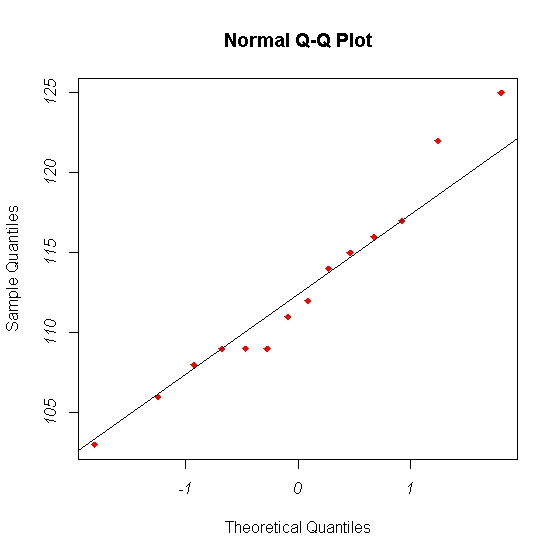
\includegraphics[scale=0.45]{images/Q5examQQplot}
%\end{center}

\begin{itemize}
	\item[i.]  Provide a brief description on how to interpret this plot.
	\item[ii.]  What is your conclusion for this procedure? Justify your answer.
\end{itemize}

\subsection*{Q5. Testing Normality (3 Marks)} %4 Marks
Consider the following inference procedure performed on data set $X$.
\begin{center}
	\begin{verbatim}
	> shapiro.test(X)
	
	Shapiro-Wilk normality test
	
	data:  X
	W = 0.9619, p-value = 0.6671
	
	\end{verbatim}
\end{center}


\begin{itemize}
	\item[i.]  Describe what is the purpose of this procedure.
	\item[ii.]  What is the null and alternative hypothesis?
	\item[iii.]  Write the conclusion that follows from it.
\end{itemize}

\subsection*{Q6. Testing For Outliers (6 Marks)}
\begin{itemize}
	\item[(i)] (3 Marks) Provide a brief description for three tests from the family of Grubb's  Outliers Tests. Include in your description a statement of the null and alternative hypothesis for each test, any required assumptions and the limitations of these tests.
	\item[(ii)] (3 Marks) Showing your working, use the Dixon Q Test to test the hypothesis that the maximum value of the following data set is an outlier.
	\[ 19,22,23,24,25,26,29,38\]
\end{itemize}
\newpage
%\newpage
\subsection*{Q2. Normal Distribution (5 Marks)} % Normal %6 MARKS
Assume that the diameter of a critical component is normally distributed with a Mean of 100mm and a Standard Deviation of 5mm. You are required  to estimate the approximate probability of the following measurements occurring on an individual component.
\begin{itemize}
	\item [i.]	Greater than 103mm
	\item [ii.] Less than 94.2 mm
	\item [iii.][$\ast$] Between 94.2 and 103 mm
\end{itemize}
\bigskip
\noindent Use the normal tables to determine the probabilities for the above exercises. You are required to show all of your workings.
\newpage
(Write Your Answers Here)
\newpage

\subsection*{Q3. Chi-Square Test (8 Marks)} %4 

A market research survey was carried out to assess preferences for three brands of chocolate bar, A, B, and C. 
The study group was categorised by gender to determine any difference in preferences.


{
	\large
	\begin{center}
		\begin{tabular}{|c|c|c|c|c|}
			\hline
			& A & B & C &  Total\\ \hline
			Females & 50 & 70 & 80 & 200 \\ \hline
			Males   & 90 & 50 & 20 &  160\\ \hline
			Total & 140 & 120 & 100 & 360\\ \hline
		\end{tabular} 
	\end{center}
}
\begin{itemize}
	\item[i.][$\ast$] Formally state the null and alternative hypotheses.
	\item[ii.]  Compute the cell values expected under the null hypothesis. Show your workings for two cells.
	\item[iii.](3 Marks) Compute the Test Statistic.
	\item[iv.][$\ast$] State the appropriate Critical Value for this hypothesis test.
	\item[v.][$\ast$] Discuss your conclusion to this test, supporting your statement with reference to appropriate values.
\end{itemize}



\newpage

\subsection*{Q8. Chi-Square Test (9 Marks)} %4 
Suppose you conducted a drug trial on a group of animals and you hypothesized that the animals receiving the drug would show increased heart rates compared to those that did not receive the drug. You conduct the study and collect the following data:
{
	\large
\begin{center}
\begin{tabular}{|c|c|c|c|}
	\hline  & Heart Rate & No Heart Rate  &  \\  
	  & Increased & Increase & Increase \\ 
	\hline Treated  & 36 & 14 & 50 \\ 
	\hline Not Treated & 30 & 25 & 55 \\ 
	\hline  & 66 & 39 & 105 \\ 
	\hline 
\end{tabular} 
\end{center}
}
\begin{itemize}
	\item[i.] Formally state the null and alternative hypotheses.
	\item[ii.]  Compute the cell values expected under the null hypothesis. Show your workings for two cells.
	\item[iii.](3 Marks) Compute the Test Statistic.
	\item[iv.] State the appropriate Critical Value for this hypothesis test.
	\item[v.] Discuss your conclusion to this test, supporting your statement with reference to appropriate values.
\end{itemize}

%\end{itemize}
% -- Part 2 - Hypothesis Testing Computation
%
% 1 Mark
% 1 Mark
%Compute the pooled variance for the aggregate sample
% 1 Mark Standard Error
% 1 Mark Test Statistic
% 1 Mark Appropriate level of significance
% 1 Mark Appropriate degrees of freedom
% 1 Mark Appropriate Critical value
% 1 MArk Discuss your conclusion to this test, supporting your statement with reference to appropriate values.

\newpage


\section*{Formulae and Tables}
\subsection*{Critical Values for Dixon Q Test}
{
	\Large
	\begin{center}
		\begin{tabular}{|c|c|c|c|}
			\hline  N  & $\alpha=0.10$  & $\alpha=0.05$  & $\alpha=0.01$  \\ \hline
			3  & 0.941 & 0.97  & 0.994 \\ \hline
			4  & 0.765 & 0.829 & 0.926 \\ \hline
			5  & 0.642 & 0.71  & 0.821 \\ \hline
			6  & 0.56  & 0.625 & 0.74  \\ \hline
			7  & 0.507 & 0.568 & 0.68  \\ \hline
			8  & 0.468 & 0.526 & 0.634 \\ \hline
			9  & 0.437 & 0.493 & 0.598 \\ \hline
			10 & 0.412 & 0.466 & 0.568 \\ \hline
			11 & 0.392 & 0.444 & 0.542 \\ \hline
			12 & 0.376 & 0.426 & 0.522 \\ \hline
			13 & 0.361 & 0.41  & 0.503 \\ \hline
			14 & 0.349 & 0.396 & 0.488 \\ \hline
			15 & 0.338 & 0.384 & 0.475 \\ \hline
			16 & 0.329 & 0.374 & 0.463 \\ \hline
		\end{tabular} 
	\end{center}
}
\subsection*{Critical Values for Chi Square Test}
{
	\Large
	\begin{center}
		\begin{tabular}{|c|c|c|c|c|}
			\hline 
			n	&	$\alpha=0.10$	&	$\alpha=0.05$	&	$\alpha=0.01$	&	$\alpha=0.001$	\\ \hline
			1	& 	2.705	&	3.841	&	6.634	&	10.827	\\ \hline
			2	&	4.605	&	5.991	&	7.378	&	9.21	\\ \hline
			3	&	6.251	&	7.815	&	9.348	&	11.345	\\ \hline
			4	&	7.779	&	9.488	&	11.143	&	13.277	\\ \hline
			5	&	9.236	&	11.07	&	12.833	&	15.086	\\ \hline
			6	&	10.645	&	12.592	&	14.449	&	16.812	\\ \hline
			7	&	12.017	&	14.067	&	16.013	&	18.475	\\ \hline
			8	&	13.362	&	15.507	&	17.535	&	20.09	\\ \hline
			9	&	14.684	&	16.919	&	19.023	&	21.666	\\ \hline
			10	&	15.987	&	18.307	&	20.483	&	23.209	\\ \hline
		\end{tabular} 
	\end{center}
}
\newpage
\subsection*{Test Statistic for Chi-Square Test}
{
\Large
\[ \chi^2_{TS} = \sum \frac{(\mbox{Observed} -\mbox{Expected} )^2}{\mbox{Expected} }\]
}


\subsection*{Confidence Intervals}
{\bf One sample}
\begin{eqnarray*} S.E.(\bar{X})&=&\frac{\sigma}{\sqrt{n}}.\\\\
S.E.(\hat{P})&=&\sqrt{\frac{\hat{p}\times(100-\hat{p})}{n}}.\\
\end{eqnarray*}
{\bf Two samples}
\begin{eqnarray*}
S.E.(\bar{X}_1-\bar{X}_2)&=&\sqrt{\frac{\sigma^2_1}{n_1}+\frac{\sigma_2^2}{n_2}}.\\\\
S.E.(\hat{P_1}-\hat{P_2})&=&\sqrt{\frac{\hat{p}_1\times(100-\hat{p}_1)}{n_1}+\frac{\hat{p}_2\times(100-\hat{p}_2)}{n_2}}.\\\\
\end{eqnarray*}
\subsection*{Hypothesis tests}
{\bf One sample}
\begin{eqnarray*}
S.E.(\bar{X})&=&\frac{\sigma}{\sqrt{n}}.\\\\
S.E.(\pi)&=&\sqrt{\frac{\pi\times(100-\pi)}{n}}
\end{eqnarray*}
{\bf Two large independent samples}
\begin{eqnarray*}
S.E.(\bar{X}_1-\bar{X}_2)&=&\sqrt{\frac{\sigma^2_1}{n_1}+\frac{\sigma_2^2}{n_2}}.\\\\
S.E.(\hat{P_1}-\hat{P_2})&=&\sqrt{\left(\bar{p}\times(100-\bar{p})\right)\left(\frac{1}{n_1}+\frac{1}{n_2}\right)}.\\
\end{eqnarray*}
{\bf Two small independent samples}
\begin{eqnarray*}
S.E.(\bar{X}_1-\bar{X}_2)&=&\sqrt{s_p^2\left(\frac{1}{n_1}+\frac{1}{n_2}\right)}.\\\\
s_p^2&=&\frac{s_1^2(n_1-1)+s_2^2(n_2-1)}{n_1+n_2-2}.\\
\end{eqnarray*}
{\bf Paired sample}
\begin{eqnarray*}
S.E.(\bar{d})&=&\frac{s_d}{\sqrt{n}}.\\\\
\end{eqnarray*}
{\bf Standard Deviation of case-wise differences (computational formula)}
\begin{eqnarray*}
s_d = \sqrt{ {\sum d_i^2 - n\bar{d}^2 \over n-1}}.\\\\
\end{eqnarray*}
\subsection*{Q1. Theory for Inference Procedures }
Answer the following short questions. Each correct answer will be awarded 1 mark.
\begin{itemize}
	% \item[i.] What is a $p-$value?
	%\item[i.] Briefly describe how $p-$value is used in hypothesis testing
	\item[i.](1 Marks)[$\ast$] What is meant by a Type I error?
	\item[ii.](1 Marks)[$\ast$] What is meant by a Type II error?
\end{itemize}
% -- Part 1 - Theory
%
% 1 Mark What is a $p-$value
% 1 Mark Briefly describe how $p-$value is used in hypothesis testing
% 1 Mark Type I error
% 1 Mark Type II error
% 2 Marks A data set is determined to be not normally distributed. Briefly describe two operations that can typically be performed in this instance.
% -- Log Transformation
% -- Test for Outliers
% 1 Mark Non Parametric Inference
% -- Marks Tally so far 7 Marks




\section*{Question 1. (25 marks) Descriptive Statistics}
\subsubsection*{Part A - Graphical Methods (15 Marks)} %28 MARKS
The exam results for a class of 40 students are tabulated below.
\begin{table}[ht]
	\begin{center}
		\begin{tabular}{|rrrrrrrrrr|}
			\hline
		%	  32 &  33 &  34 &  36 &  36 &  37 &  37 &  38 &  38 &  38 \\ 
			  32 &  33 &  34 &  36 &  43 &  44 &  44 &  44 &  45 &  46 \\ 
		      47 &  47 &  48 &  49 &  49 &  49 &  49 &  50 &  51 &  52 \\ 
			  52 &  53 &  53 &  53 &  55 &  56 &  57 &  59 &  60 &  62 \\ 
		%	  59 &  59 &  59 &  61 &  61 &  62 &  64 &  64 &  64 &  65 \\ 
			  65 &  65 &  67 &  70 &  75 &  79 &  81 &  83 &  87 &  91 \\ 		\hline
		\end{tabular}
	\end{center}
\end{table}
\vspace{-0.5cm}
\begin{enumerate}[(i)]
	\item (3 Marks) Summarize the data in the above table using a relative frequency table, a cumulative frequency table, and a cumulative relative frequency table. Use 7 class intervals, with 31 as the lower limit of the first interval.
	\item (6 Marks) Draw a histogram for the above data. Comment on the shape of the histogram. Based on the shape of the histogram, what is the best measure of centrality and variability?
	\item (6 Marks) Construct a box plot for the above data. Clearly demonstrate how all of the necessary values were computed.
\end{enumerate}


\subsection*{Part B - Dixon Q Test (5 Marks)}

	
	Use the Dixon Q-test to determine if the highest value is an outlier. You may assume a significance level of 5\%.
		\[ 17,20,23,24,25,26,28,45\]
	\begin{itemize}
		\item[(i)](1 Mark) State the null and alternative hypotheses for this test.
		\item[(ii)](2 Marks) Compute the test statistic.
		\item[(iii)](1 Mark) State the appropriate critical value.
		\item[(iv)](1 Mark) What is your conclusion to this procedure.
	\end{itemize}

\vspace{0.25cm}
\subsection*{Part C - Summary Statistics (5 Marks)} %10 MARKS
Data on the durations (measured in months) were collected for a random sample of product development projects. The durations for these development projects are as follows:

\begin{table}[ht]
	\centering
	\begin{tabular}{|rrrrrrrrr|}
		\hline
		
		18& 20& 26& 18& 21& 19& 29& 21& 17\\ 
		\hline
	\end{tabular}
\end{table}
\vspace{-0.5cm}


\begin{enumerate}[(i)]
	\item (1 Mark) Calculate the mean project duration.
	\item (1 Mark) Compute the median project duration.
	\item (2 Marks) Calculate the variance of the project durations.
	\item (1 Mark) Calculate the standard deviation of the project durations.
\end{enumerate}

%\subsection*{Part A - Boxplots (6 Marks)}
%Construct a pair of box plots for the data in the below. Construct one box plot for the data related to Material A, the other for Material B. Comment on the features of the box plots and what conclusions, if any, you can derive from the two box plots.
%\begin{center}
%	\begin{tabular}{|c|c|l|}
%		\hline
%		Material & Sample size & Bonding Strength (Newton Metres) \\ \hline
%		
%		A (80\% pure) & 12 & 2.0 2.1 2.1 2.1 2.2 2.3 2.3 2.3 2.4 2.4 2.5 2.6
%		\\ \hline
%		
%		B (60\% pure) & 10 & 1.9 1.9 2.0 2.1 2.1 2.2 2.2 2.5 2.7 2.8 \\ \hline
%	\end{tabular} 
%\end{center}
%\medskip
%\textit{
%	\noindent Marking Scheme:
%	\begin{itemize}
%		\item 4 Marks for showing the relevant calculations,
%		\item 1 Mark for drawing the boxplots to a satisfactory standard.
%		\item 1 Mark for a well-explained conclusion,
%	\end{itemize}
%}
\newpage



\section*{Question 2. (25 marks) Probability Distributions }




\subsection*{Part A - Normal Distribution (10 Marks)}

\smallskip	
\noindent Assume that the diameter of a critical component is normally distributed with a mean of 1002mm and a standard deviation of 1.25mm. You are required  to estimate the approximate probability of the following measurements occurring on an individual component.
\begin{itemize}
	\item[(i)](2 Mark) Greater than 1004.3mm.
	\item[(ii)](3 Marks) Less than 1000mm.
	\item [(iii)](2 Marks) Between 1000mm and 1004mm.
	\item[(iv)] (3 Marks) The production manager reports that more than 99\% of the output is between 998mm and 1004mm. Do you agree with this statement? Justify your answer with the appropriate calculations.
\end{itemize}
\medskip
\noindent Use statistical tables to determine the probabilities for the above exercises. You are required to show all of your workings.

\bigskip
\subsection*{Part B - Probability (10 Marks)} % Normal %6 MARKS
A new test has been developed to diagnose a particular disease. If a person has the disease, the test has a 95\% chance of identifying them as having the disease.
If a person does not have the disease, the test has a 1\% chance of identifying them as having the disease.  Suppose that 5\% of the population have this disease. Suppose we select a person at random from the population.


\begin{enumerate}[(i)]
	\item (4 Marks) What is the probability that the test will identify them as having the disease?
	
	\item (3 Marks) What is the probability that the person has the disease given that the test identifies them as having the disease?
	\item (3 Marks) What is the probability that the person has the disease given that the test identifies them as \textbf{not} having the disease?
\end{enumerate}

\subsection*{Part C - Testing Distributional Assumptions (5 Marks)}
Consider the results of a statistical analysis carried out on sample data for the random variable $Y$. These results are presented as output from a statistical computing program.

\begin{itemize}
	\item[(i)] (1 Mark) What sort of statistical analysis are we carrying out? 
	\item[(ii)] (1 Mark) What is the relevance of this analysis as part of an overall statistical study.
	\item[(ii)] (2 Mark) Interpret the output of the Anderson-Darling Test. (\textit{Remark: Use a 5\% significance level. This test is a one-tailed procedure.})
	\item[(iv)] (1 Mark) What is the conclusion of this analysis for the variable $Y$? Justify your answer with reference to 3 separate indications. 
	
\end{itemize}
\noindent (\textit{Computer results continue on the next page.})
%\bigskip
%\textit{\textbf{Important:} Question 3 comprises a third part: Part C. This part is presented in subsequent pages.}

\begin{figure}[h!]
	\centering
	\includegraphics[width=0.99\linewidth]{images/NormalityTesting3}
\end{figure}
\begin{figure}[h!]
	\centering
	\includegraphics[width=0.99\linewidth]{images/NormalityTesting4}
\end{figure}

\newpage


%=================================================================%


\section*{Question 3. (25 marks) Single Sample Inference Procedures }

\subsection*{Part A - Inference Procedures for Proportion (10 Marks)}
%% Change the Numbers

The conventional treatment for a disease has been shown to be effective in 65\% of all 
cases. A new drug has been developed by a pharmaceutical company. The Health Service Executive of Ireland
wishes to determine whether the new treatment is more effective than conventional treatment. 
A simple random sample of 400 patients are given the new drug. The treatment is effective for 200 of them.
% You are required to make a recommendation about purchasing the new drug.


\begin{itemize}
	\item[(i)](6 Marks) Compute the 95\% confidence interval.
%	\item[(ii)](3 Marks) Compute the Test Statistic.
	\item[(ii)](4 Marks) By interpreting this confidence interval, make a recommendatiion about purchasing the new drug? Explain how you made this decision.
\end{itemize}
%======================================================================%

\subsection*{Part B - Inference Procedures for the Mean (15 Marks)}
Mean blood iron concentration for children with adequate nutrition is taken to be 110mg/dl. \\ \smallskip


\noindent 50 randomly selected children from a disadvantaged urban area were given blood tests. The mean concentration of iron from this sample was 98 mg/dl with a standard deviation of 25.5 mg/dl.
\begin{itemize}
	\item[(i)] (4 Marks) Calculate a 95\% confidence interval for the mean concentration of iron for children in this area. 
	\item[(ii)](2 Marks) Interpret this confidence interval.  Do these results provide evidence that children in this area suffer from iron deficiency? 
\end{itemize}
\medskip
Test this hypothesis using a 5\% level of significance. 

\begin{itemize}
	\item[(iii)](3 Marks) Clearly state your null and alternative hypotheses.
	\item[(iv)](4 Marks) Compute the test statistic.
	\item[(v)](2 Marks) Discuss your conclusion to this test, supporting your statement with reference to appropriate values.
\end{itemize}


\newpage



\section*{Question 4. (25 marks) Two Sample Inference Procedures}

\subsection*{Part A - Two Sample $t-$ Test (10 Marks)}

An exercise physiologist wants to determine if several short bouts of exercise provide the same benefit for cardiovascular fitness as one long bout of exercise. \\ \smallskip

\noindent 60 volunteers are randomly assigned to group 1 and do standardised aerobic exercise on a stationary bicycle for 30 minutes once a day, 5 days a week. 40 volunteers are randomly assigned to group 2 and do the same exercise for 10 minutes, 3 times a day, 5 days a week. Cardiovascular fitness was measured by VO2 max (maximum oxygen consumption while exercising). 

\begin{description}
	\item[Group 1] The mean change in VO2 after 12 weeks of exercise was 2.1 for group 1 with a standard deviation of 1.7.
	\item[Group 2] The mean change in VO2 after 12 weeks of exercise was 0.7 for group 2 with a standard deviation of 1. 
\end{description}

\noindent Test the hypothesis that there is no significant difference between two groups are the same.

\begin{itemize}
	\item[(i)](3 Marks) Formally state your null and alternative hypotheses.
	\item[(ii)](4 Marks) Compute the test statistic.
	\item[(iii)](3 Marks) Discuss your conclusion to this test, supporting your statement with reference to appropriate values.
\end{itemize}


\subsection*{Part B - Inferences for Differences in Proportions (15 Marks)}
A survey of 1000 Irish indicates that 700 have access to the Internet. A survey of 1200 Czechss
indicates that 700 have access to the Internet.
\begin{itemize}
	\item[(i)] (3 marks) Provide an estimate of the difference between the population
	proportions (i.e. $\pi_l -\pi_2$).
	
	\item[(ii)] (7 marks) Test the hypothesis that the proportion of all Irish
	having access to the Internet is equal to the proportion of all Czechs having access to the
	internet at a significance level of 5%.
	
	\item[(iii)] (5 marks) Calculate a 95\% confidence interval for the difference between the proportion of all Irish
	having access to the Internet and the proportion of all Czechs having access to the
	internet.
	
	
\end{itemize}

%===============================================================================%
\newpage

\section*{Question 5. (25 marks) Linear Regression Models and Chi Square Tests }
\subsection*{Part A - Chi Square Tests (10 Marks)}
A market research survey was carried out to assess preferences for three brands of chocolate bar, A, B, and C. 
The study group was categorised by maturity level to determine any difference in preferences. The purpose of this study is to assess differing preferences for brands across age groups.


{
	\begin{center}
		\begin{tabular}{|c||c|c|c||c|} \hline
			&	Brand A	&	Brand B	&	Brand C	&	Total	\\ \hline		\hline
			Children	&	65	&	55	&	30	&	150	\\ \hline	
			Teenages	&	35	&	75	&	40	&	150	\\ \hline	
			Adults	&	50	&	20	&	30	&	100	\\ \hline	\hline
			&	150	&	150	&	100	&	400	\\ \hline	 
		\end{tabular} 
	\end{center}
}
\begin{enumerate}[(i)]
	\item (1 Mark) Formally state the null and alternative hypotheses.
	\item (2 Marks) Compute each of the cell values expected under the null hypothesis. 
	\item (4 Marks) Compute the test statistic.
	\item (1 Mark) State the appropriate critical value for this hypothesis test.
	\item (2 Marks) Discuss your conclusion to this test, supporting your statement with reference to appropriate values.
\end{enumerate}




\subsection*{Part B - Linear Regression (15 Marks)}

An experiment was conducted to study the relationship between baking temperature x (in units of 10 degrees Farenheit) and yield y (as percentage) of popular cake mix. Fourteen observations were made giving the following results.

%Temp 10 10.5 11 11.5 12 15 17 19 20 21 23 25 27 30

%Yield 21.2 19.9 22.5 23.7 25 30.3 36.1 38.6 41.5 42.7 45 50 53.9 62.1



\begin{center}
	\begin{tabular}{|c||c|c|c|c|c|c|c|}
		\hline
		Specimen & 1 & 2 & 3 & 4 & 5 & 6 & 7 \\ \hline
		\hline
		Temp &  10.00 & 10.50 & 11.00 & 11.50 & 12.00 & 15.00 & 17.00 \\ \hline 
		Yield &  29.830&  26.370 & 30.325 &36.100 &33.410 &36.335 & 40.655 \\ \hline 
		\hline\hline
		Specimen & 8 & 9 & 10 & 11 & 12 & 13 & 14 \\  \hline
		Temp &  19.00 & 20.00 & 21.00 & 23.00 & 25.00 & 27.00 & 30.00 \\ \hline
		Yield &  39.475& 44.555&  42.015 & 47.795 & 45.560&  51.045 & 47.900 \\ \hline 
		\hline
	\end{tabular}
\end{center}

\begin{multicols}{3}
	\begin{itemize}
		\item $S_{XX} = 570.5$
		\item $S_{YY} =  751.1525$
		\item $S_{XY} = 613.27$
		\item $\bar{X} = 18$
		\item $\bar{Y} = 39.383$
	\end{itemize}
\end{multicols}
\medskip
\textit{(This question is continued on the next page.)}
\newpage

\begin{figure}
\centering
\includegraphics[width=0.99\linewidth]{images/MA4603-Regression-Repeat}
\caption{}
\label{fig:ma4603-regression-repeat}
\end{figure}
\medskip
\begin{enumerate}[(i)]
	
	\item (2 Marks) Using the scatter plot, describe the relationship between the yield (Y) and the baking temperature (X).
	
	
	
	
	
	\item (4 Marks) Calculate the correlation coefficient. Interpret your answer.
	\item (6 Marks) Calculate the equation of the least squares regression line and interpret the value of the slope.
	\item (3 Marks) Using this regression model, estimate the yield when the baking temperature is 16 degrees.
	%		\item (2 Marks) How much of the variation in yield is explained by fitting the regression line?
\end{enumerate}

\newpage


\section*{Formulae}
%-------------------------------------------------%
\subsection*{Descriptive Statistics}
\begin{itemize}
	\item Sample Variance
	\begin{equation*}
	s^2 = \frac{\sum (x-\bar{x})^2}{n-1}
	\end{equation*}
\end{itemize}
%-------------------------------------------------%
\subsection*{Probability}
\begin{itemize}
	
	\item Conditional probability:
	\begin{equation*}
	P(B|A)=\frac{P\left( A\text{ and }B\right) }{P\left( A\right) }.
	\end{equation*}
	
	
	\item Bayes' Theorem:
	\begin{equation*}
	P(B|A)=\frac{P\left(A|B\right) \times P(B) }{P\left( A\right) }.
	\end{equation*}
	
	
	
	
	%	
	%	\item Binomial probability distribution:
	%	\begin{equation*}
	%		P(X = k) = ^{n}C_{k} \times p^{k} \times \left( 1-p\right) ^{n-k}\qquad \left( \text{where  }
	%		^{n}C_{k} =\frac{n!}{k!\left(n-k\right) !}. \right)
	%	\end{equation*}
	%	
	%	\item Poisson probability distribution:
	%	\begin{equation*}
	%		P(X = k) =\frac{m^{k}\mathrm{e}^{-m}}{k!}.
	%	\end{equation*}
	%	
	%	\item Exponential probability distribution:
	%	\begin{equation*}
	%		P(X \leq k) = \begin{cases}
	%			1-e^{- k/\mu}, & k \ge 0, \\
	%			0, & k < 0.
	%		\end{cases}\qquad \left( \text{where  }
	%		\mu = {1\over \lambda}\right)
	%	\end{equation*}
\end{itemize}

\subsection*{Confidence Intervals}
{\bf One sample}
\begin{eqnarray*} S.E.(\bar{X})&=&\frac{\sigma}{\sqrt{n}}.\\\\
	S.E.(\hat{P})&=&\sqrt{\frac{\hat{p}\times(1-\hat{p})}{n}}.\\
\end{eqnarray*}
{\bf Two samples}
\begin{eqnarray*}
	S.E.(\bar{X}_1-\bar{X}_2)&=&\sqrt{\frac{\sigma^2_1}{n_1}+\frac{\sigma_2^2}{n_2}}.\\\\
	S.E.(\hat{P_1}-\hat{P_2})&=&\sqrt{\frac{\hat{p}_1\times(1-\hat{p}_1)}{n_1}+\frac{\hat{p}_2\times(100-\hat{p}_2)}{n_2}}.\\\\
\end{eqnarray*}
\subsection*{Hypothesis tests}
{\bf One sample}
\begin{eqnarray*}
	S.E.(\bar{X})&=&\frac{\sigma}{\sqrt{n}}.\\\\
	S.E.(p)&=&\sqrt{\frac{p \times(1-p)}{n}}
\end{eqnarray*}
{\bf Two large independent samples}
\begin{eqnarray*}
	S.E.(\bar{X}_1-\bar{X}_2)&=&\sqrt{\frac{\sigma^2_1}{n_1}+\frac{\sigma_2^2}{n_2}}.\\\\
	S.E.(\hat{P_1}-\hat{P_2})&=&\sqrt{\left(\bar{p}\times(1-\bar{p})\right)\left(\frac{1}{n_1}+\frac{1}{n_2}\right)}.\\
\end{eqnarray*}
{\bf Two small independent samples}
\begin{eqnarray*}
	S.E.(\bar{X}_1-\bar{X}_2)&=&\sqrt{s_p^2\left(\frac{1}{n_1}+\frac{1}{n_2}\right)}.\\\\
	s_p^2&=&\frac{s_1^2(n_1-1)+s_2^2(n_2-1)}{n_1+n_2-2}.\\
\end{eqnarray*}
{\bf Paired sample}
\begin{eqnarray*}
	S.E.(\bar{d})&=&\frac{s_d}{\sqrt{n}}.\\\\
\end{eqnarray*}
{\bf Standard Deviation of case-wise differences (computational formula)}
\begin{eqnarray*}
	s_d = \sqrt{ {\sum d_i^2 - n\bar{d}^2 \over n-1}}.\\\\
\end{eqnarray*}
\subsection*{Chi Square Tests of Independence}
\[\chi^2_{TS} =  \sum \frac{(n_{ij} - e_{ij})^2}{e_{ij}}\]
\subsection*{Regression Estimates}
\begin{eqnarray*}
	S_{XY} &=&
	\sum x_iy_i - \frac{\sum x_i\sum y_i}{n}\\
	S_{XX} &=&
	\sum x_i^2 - \frac{(\sum x_i)^2}{n}\\
	S_{YY} &=&
	\sum y_i^2 - \frac{(\sum y_i)^2}{n}\\
\end{eqnarray*}
{\bf Pearson's correlation coefficient}

\begin{eqnarray*}
	r = \frac{S_{XY}}{\sqrt{S_{XX} \times S_{YY}}}
\end{eqnarray*}
{\bf Slope Estimate}
\begin{eqnarray*}
	b_1 = \frac{S_{XY}}{S_{XX}}
\end{eqnarray*}
{\bf Intercept Estimate}
\begin{eqnarray*}
	b_0 = \bar{y} -b_1\bar{x}
\end{eqnarray*}



\section*{Question 1. (25 marks) Descriptive Statistics}
\subsubsection*{Part A - Graphical Methods (15 Marks)} %28 MARKS
The exam results for a class of 60 students are tabulated below.
\begin{table}[ht]
	\begin{center}
		\begin{tabular}{|rrrrrrrrrr|}
			\hline
			  15 &  28 &  29 &  31 &  33 &  35 &  36 &  38 &  38 &  38 \\ 
			  39 &  40 &  41 &  42 &  43 &  44 &  44 &  44 &  45 &  45 \\ 
			  45 &  46 &  47 &  48 &  48 &  48 &  48 &  48 &  50 &  52 \\ 
			  52 &  53 &  53 &  53 &  54 &  55 &  57 &  57 &  58 &  58 \\ 
			  59 &  59 &  59 &  61 &  61 &  62 &  64 &  64 &  64 &  65 \\ 
			  65 &  65 &  67 &  67 &  68 &  70 &  72 &  80 &  81 &  89 \\ 		\hline
		\end{tabular}
	\end{center}
\end{table}
\vspace{-0.5cm}
\begin{enumerate}[(i)]
	\item (3 Marks) Summarize the data in the above table using a relative frequency table, a cumulative frequency table, and a cumulative relative frequency table. Use 8 class intervals, with 11 as the lower limit of the first interval.
	\item (6 Marks) Draw a histogram for the above data. Comment on the shape of the histogram. Based on the shape of the histogram, what is the best measure of centrality and variability?
	\item (6 Marks) Construct a box plot for the above data. Clearly demonstrate how all of the necessary values were computed.
\end{enumerate}

\vspace{0.25cm}
\subsubsection*{Part B - Summary Statistics (5 Marks)} %10 MARKS
Data on the durations (measured in months) were collected for a random sample of product development projects. The durations for these development projects are as follows:

\begin{table}[ht]
	\centering
	\begin{tabular}{|rrrrrrrr|}
		\hline
		
		21 &  13 &  16 &  11 &  16 &  16 &  21 &  22 \\ 
		\hline
	\end{tabular}
\end{table}
\vspace{-0.5cm}


\begin{enumerate}[(i)]
	\item (1 Mark) Calculate the mean project duration.
	\item (1 Mark) Compute the median project duration.
	\item (2 Marks) Calculate the variance of the project durations.
	\item (1 Mark) Calculate the standard deviation of the project durations.
\end{enumerate}

%\subsection*{Part A - Boxplots (6 Marks)}
%Construct a pair of box plots for the data in the below. Construct one box plot for the data related to Material A, the other for Material B. Comment on the features of the box plots and what conclusions, if any, you can derive from the two box plots.
%\begin{center}
%	\begin{tabular}{|c|c|l|}
%		\hline
%		Material & Sample size & Bonding Strength (Newton Metres) \\ \hline
%		
%		A (80\% pure) & 12 & 2.0 2.1 2.1 2.1 2.2 2.3 2.3 2.3 2.4 2.4 2.5 2.6
%		\\ \hline
%		
%		B (60\% pure) & 10 & 1.9 1.9 2.0 2.1 2.1 2.2 2.2 2.5 2.7 2.8 \\ \hline
%	\end{tabular} 
%\end{center}
%\medskip
%\textit{
%	\noindent Marking Scheme:
%	\begin{itemize}
%		\item 4 Marks for showing the relevant calculations,
%		\item 1 Mark for drawing the boxplots to a satisfactory standard.
%		\item 1 Mark for a well-explained conclusion,
%	\end{itemize}
%}
\newpage
\subsection*{Part C - Dixon Q Test (5 Marks)}

	
	Use the Dixon Q-test to determine if the lowest value is an outlier. You may assume a significance level of 5\%.
		\[ 11,22,23,24,25,26,29,34\]
	\begin{itemize}
		\item[(i)](1 Mark)	State the null and alternative hypotheses for this test.
		\item[(ii)](2 Marks) Compute the test statistic.
		\item[(iii)](1 Mark) State the appropriate critical value.
		\item[(iv)](1 Mark) What is your conclusion to this procedure.
	\end{itemize}



\section*{Question 2. (25 marks) Probability Distributions }




\subsection*{Part A - Normal Distribution (10 Marks)}

\smallskip	
\noindent Assume that the diameter of a critical component is normally distributed with a mean of 1000mm and a standard deviation of 1.25mm. You are required  to estimate the approximate probability of the following measurements occurring on an individual component.
\begin{itemize}
	\item[(i)](2 Mark) Greater than 1001.7mm.
	\item[(ii)](3 Marks) Less than 998.1mm.
	\item [(iii)](2 Marks) Between 998.1mm and 1002.3mm.
	\item[(iv)] (3 Marks) The production manager reports that more than 99\% of the output is between 997mm and 1003mm. Do you agree with this statement? Justify your answer with the appropriate calculations.
\end{itemize}
\medskip
\noindent Use statistical tables to determine the probabilities for the above exercises. You are required to show all of your workings.

\bigskip
\subsection*{Part B - Probability (10 Marks)} % Normal %6 MARKS
A new test has been developed to diagnose a particular disease. If a person has the disease, the test has a 95\% chance of identifying them as having the disease.
If a person does not have the disease, the test has a 1\% chance of identifying them as having the disease.  Suppose that 5\% of the population have this disease. Suppose we select a person at random from the population.


\begin{enumerate}[(i)]
	\item (4 Marks) What is the probability that the test will identify them as having the disease?
	
	\item (3 Marks) What is the probability that the person has the disease given that the test identifies them as having the disease?
	\item (3 Marks) What is the probability that the person has the disease given that the test identifies them as \textbf{not} having the disease?
\end{enumerate}

\subsection*{Part C - Testing Distributional Assumptions (5 Marks)}
Consider the results of a statistical analysis carried out on sample data for the random variable $X$. These results are presented as output from a statistical computing program.

\begin{itemize}
	\item[(i)] (1 Mark) What sort of statistical analysis are we carrying out? 
	\item[(ii)] (1 Mark) What is the relevance of this analysis as part of an overall statistical study.
	\item[(ii)] (2 Mark) Interpret the output of the Anderson-Darling Test. (\textit{Remark: Use a 5\% significance level. This test is a one-tailed procedure.})
	\item[(iv)] (1 Mark) What is the conclusion of this analysis for the variable $X$? Justify your answer with reference to 3 separate indications. 
	
\end{itemize}
\noindent (\textit{Computer results continue on the next page.})


\begin{figure}[h!]
	\centering
	\includegraphics[width=0.99\linewidth]{images/NormalityTesting1}
\end{figure}
\begin{figure}[h!]
	\centering
	\includegraphics[width=0.99\linewidth]{images/NormalityTesting2}
\end{figure}

\newpage




%=================================================================%


\section*{Question 3. (25 marks) Single Sample Inference Procedures }
\subsubsection*{Part A - Single Sample Inference Procedures (15 Marks)}
Mean blood iron concentration for children with adequate nutrition is taken to be 110mg/dl. \\ \smallskip


\noindent 25 randomly selected children from a disadvantaged urban area were given blood tests. The mean concentration of iron from this sample was 98 mg/dl with a standard deviation of 25.5 mg/dl.
\begin{itemize}
	\item[(i)] (4 Marks) Calculate a 95\% confidence interval for the mean concentration of iron for children in this area. 
	\item[(ii)](2 Marks) Interpret this confidence interval.  Do these results provide evidence that children in this area suffer from iron deficiency? 
\end{itemize}
\medskip
Test this hypothesis using a 5\% level of significance. 

\begin{itemize}
	\item[(iii)](3 Marks) Clearly state your null and alternative hypotheses.
	\item[(iv)](4 Marks) Compute the test statistic.
	\item[(v)](2 Marks) Discuss your conclusion to this test, supporting your statement with reference to appropriate values.
\end{itemize}


\newpage

\subsection*{Part B - Single Sample Proportion (10 Marks)}
%% Change the Numbers

The conventional treatment for a disease has been shown to be effective in 60\% of all 
cases. A new drug has been developed by a pharmaceutical company. The Health Service Executive of Ireland
wishes to determine whether the new treatment is more effective than conventional treatment. 
A simple random sample of 400 patients are given the new drug. The treatment is effective for 300 of them.
% You are required to make a recommendation about purchasing the new drug.


\begin{itemize}
	\item[(i)](6 Marks) Compute the 95\% confidence interval.
%	\item[(ii)](3 Marks) Compute the Test Statistic.
	\item[(ii)](4 Marks) By interpreting this confidence interval, make a recommendatiion about purchasing the new drug? Explain how you made this decision.
\end{itemize}
%======================================================================%




\section*{Question 4. (25 marks) Two Sample Inference Procedures}

\subsection*{Part A - Two Sample $t-$ Test (10 Marks)}
A test of a specific blood factor has been devised such that, for adults in Western Europe, the test score is normally distributed with mean 100 and standard deviation 10. A clinical research organization is carrying out research on the blood factor levels for sufferers of a particular disease.  

\begin{itemize}
	\item A study has obtained the following test scores for 14 randomly selected patients suffering from the disease in Ireland 
	\[ \{115, 113, 111, 109, 115, 108, 121, 114, 104, 113, 122, 90, 
	103, 116\}\]
	
	\item A similar study has obtained the following test scores for 15 randomly selected patients suffering from the disease in Germany .
	\[\{120, 137, 114, 120, 116, 118, 101, 110, 125, 113, 111, 128, 
	119, 117, 121\}\]
	
	\end{itemize}
	
		\begin{center}	
	\begin{tabular}{|c|c|c|c|} \hline 
		Sample & Mean & Std. Deviation & Sample Size \\  \hline 
		Ireland & 111 & 8.143 & 14 \\ \hline 
		Gemany & 118 & 8.350 & 15 \\ \hline
		\end{tabular} 
				\end{center}
You believe that there may be a difference in blood factor levels between the two countries. Test this hypothesis using a 5\% level of significance. 
\begin{itemize}
	\item[(i)](3 Marks) Clearly state your null and alternative hypotheses.

	\item[(ii)] (2 Marks) Comput the pooled standard deviation.
	\item[(iii)](2 Marks) Compute the test statistic.
	\item[(iv)](3 Marks) Discuss your conclusion to this test, supporting your statement with reference to appropriate values.
\end{itemize}				

\subsection*{Part B - Paired T Test (15 Marks)}
In preparation for space exploration, 10 crew members underwent intensive
 medical examinations pre-flight and post-flight. As part of the examination
 of the cardiovascular system, the lower body was subjected to a pressure lower
 than that of the atmosphere by being placed in a chamber, with an airtight
 seal, connected to a vacuum source. \\ \smallskip
 
\noindent Heart rates, in beats per minute, were
 recorded when a pressure of 6700 Nm$^{−2}$ below atmospheric had been reached.
 A simplified version of the results is shown below:
		\begin{center}
			
		
			\begin{tabular}{|c|c|c|} \hline 
	Crew   & Heart Rate & Heart Rate \\
\phantom{spa}	member \phantom{spa}& \phantom{spa}Pre-flight\phantom{spa} & \phantom{spa}Post-Flight \phantom{spa}\\	\hline \hline
		1 & 79 & 94 \\ \hline
		2 & 83 & 90 \\ \hline
		3 & 47 & 56 \\ \hline 
		4 & 46 & 61 \\ \hline
		5 & 68 & 67 \\ \hline 
		6 & 74 & 88 \\ \hline
		7 & 68 & 64 \\ \hline 
		8 & 50 & 52 \\ \hline 
		9 & 59 & 54 \\ \hline 
		10 & 67 & 65 \\ \hline
			\end{tabular} 
		\end{center}


Using 5\% significance, test the hypothesis that the overall average heart rate
in beats per minutes has changed after the flight. 
\begin{itemize}
	\item[(i)](3 Marks) Formally state the null and alternative hypotheses.
	\item[(ii)] (3 Marks) Compute the mean and standard deviation of the case-wise differences.
	\item[(iii)](3 Marks) Compute the test statistic.
	\item[(iv)](3 Marks) State the appropriate critical value for this hypothesis test.
	\item[(v)](3 Marks) Discuss your conclusion to this test, supporting your statement with reference to appropriate values.
\end{itemize}
%\subsection*{Part C Testing Equality of Variances (5 Marks)} %4 Marks
%The standard deviations of data sets \texttt{X} and \texttt{Y} are 10 and 9 respectively. An inference procedure was carried out to assess whether or not \texttt{X} and \texttt{Y} can be assumed to have equal variance.
%\begin{itemize}
%	\item[i.](1 Mark) Formally state the null and alternative hypothesis.
%	\item[ii.](1 Mark) The Test Statistic has been omitted from the computer code output. Compute the value of the Test Statistic.
%	\item[iii.](2 Marks) What is your conclusion for this procedure? Justify your answer.
%	%\item[iv.] (1 Marks) Explain how a conclusion for this procedure can be based on the $95\%$ confidence interval.
%\end{itemize}
%
%%---- R code for Variance Test ----%
%%---- Dummy Code Included                   ----%
%\begin{framed}
%	\begin{verbatim}
%	F test to compare two variances
%	
%	data:  X and Y
%	F = ......, num df = 13, denom df = 11, p-value = 0.7349
%	alternative hypothesis: true ratio of variances is not equal to 1
%	95 percent confidence interval:
%	0.3639938 3.9475262
%	sample estimates:
%	ratio of variances
%	.......
%	\end{verbatim}
%\end{framed}

%===============================================================================%
\newpage

\section*{Question 5. (25 marks) Linear Regression Models and Chi Square Tests }

\subsubsection*{Part A - Chi Square Test of Association (15 Marks)}
The following contingency table illustrates the levels at which males and females smoke cigarettes. The figures in brackets give the expected number of observations in a cell under the hypothesis that smoking habits are independent of sex.

{

	\begin{center}
		\begin{tabular}{|c||l|l|l||c|}
			\hline
			& Non-smoker&  $<$ 10 per day &  $\geq $ 10  & \phantom{sp}Sum\phantom{sp} \\ \hline
			
			Males & 180\phantom{spa} (200)&  60\phantom{spa} (?) & 60 \phantom{spa} (?) & 300\\ \hline
			
			Females & 220\phantom{spa} (?) & 60 \phantom{spa}(?)& 20 \phantom{spa} (40) & 300\\ \hline \hline
			
			Sum & 400 & 120 & 80& 600\\ \hline
		\end{tabular} 
	\end{center}
	\phantom{spa}
}
\medskip
Test this hypothesis using a 5\% level of significance. 

\begin{enumerate}[(i)]
\item (2 Marks) What is the probability that a randomly chosen person from the sample smokes more than 10 cigarettes a day? % (1 mark)

\item (2 Marks) Given that the person chosen is a non-smoker, calculate the probability that this person is a female. %(1 mark)

\item (2 Marks) Replace the question marks with the expected number of observations in a cell under the null hypothesis. %(2 marks)
\item (2 Marks) Clearly state the null and alternative hypothesis.
\item (4 Marks) Compute the test statistic for this procedure.
\item (3 Marks) By interpreting the results of the the chi-squared test for independence, state your conclusions? % (6 marks)
\end{enumerate}
\subsection*{Part B - Simple Linear Regression (10 Marks)}


Data on body dimensions such as abdomen, hip and bicep circumference (measured in cm) were obtained from 252 men aged over 25. Their percentage of body fat was also recorded and an investigation carried out to see which body dimension variables have a strong relationship with the percentage of body fat. In this case, we look at abdomen circumference. 

\medskip
\noindent For this question, you may use the following values.
\begin{multicols}{3}
	\begin{itemize}
		\item $S_{XX} = 3514$ \item $S_{YY} = 4769$ \item  $S_{XY} = 3012$ \item $\bar{X} = 50$  \item $\bar{Y} = 100$  
	\end{itemize}
\end{multicols}
\medskip
\textit{(The question is continued on the next page.)}


%\begin{enumerate}
%	\item Describe the relationship between abdomen circumference and the percentage of body fat (pctfat) using the scatter plot below. (3 marks)
%	
%	
%	\item The value of the correlation coefficient is 0.813. Interpret this value.
%	
%	
%	
%	\item The least squares regression line is pctfat = -39.3 +
%	
%	0.631 abdomen. Interpret the values of the slope and intercept.
%	
%	\item  Use the output from Minitab below to investigate if there is a statistically significant relationship between pctfat and abdomen.
%	
%	\item  How much of the variation in the percentage of body fat is explained by
%	
%	abdomen circumference? Interpret this value.
%	
%	
%
%\end{enumerate}
\newpage
\begin{figure}[h!]
\centering
\includegraphics[width=0.99\linewidth]{images/MA4603-Regression}

\end{figure}







%
%Call:
%lm(formula = Y ~ X)
%
%Coefficients:
%(Intercept)            X  
%57.1429       0.8571  


\begin{enumerate}[(i)]
	
	\item (2 Marks) Using the scatter plot, state the relationship between abdomen circumference (X) and the percentage of body fat (Y) using the scatter plot.
	
	
	
	
	
	\item (3 Marks) Calculate the correlation coefficient. Interpret your answer.
	\item (5 Marks) Calculate the equation of the least squares regression line and interpret the value of the slope.
%	\item (2 Marks) Using this regression model, estimate the body fat when the abdomen circumference is 42cm.
%	\item (2 Marks) How much of the variation in yield is explained by fitting the regression line?
\end{enumerate}
%
%\begin{figure}
%	\centering
%	\includegraphics[width=0.99\linewidth]{images/MA4603-regression-residuals}
%	\caption{}
%	\label{fig:ma4603-regression-residuals}
%\end{figure}








%=============================================================%


\newpage

\section*{Formulae}
%-------------------------------------------------%
\subsection*{Descriptive Statistics}
\begin{itemize}
	\item Sample Variance
	\begin{equation*}
	s^2 = \frac{\sum (x-\bar{x})^2}{n-1}
	\end{equation*}
\end{itemize}
%-------------------------------------------------%
\subsection*{Probability}
\begin{itemize}
	
	\item Conditional probability:
	\begin{equation*}
	P(B|A)=\frac{P\left( A\text{ and }B\right) }{P\left( A\right) }.
	\end{equation*}
	
	
	\item Bayes' Theorem:
	\begin{equation*}
	P(B|A)=\frac{P\left(A|B\right) \times P(B) }{P\left( A\right) }.
	\end{equation*}
	
	
	
	
	%	
	%	\item Binomial probability distribution:
	%	\begin{equation*}
	%		P(X = k) = ^{n}C_{k} \times p^{k} \times \left( 1-p\right) ^{n-k}\qquad \left( \text{where  }
	%		^{n}C_{k} =\frac{n!}{k!\left(n-k\right) !}. \right)
	%	\end{equation*}
	%	
	%	\item Poisson probability distribution:
	%	\begin{equation*}
	%		P(X = k) =\frac{m^{k}\mathrm{e}^{-m}}{k!}.
	%	\end{equation*}
	%	
	%	\item Exponential probability distribution:
	%	\begin{equation*}
	%		P(X \leq k) = \begin{cases}
	%			1-e^{- k/\mu}, & k \ge 0, \\
	%			0, & k < 0.
	%		\end{cases}\qquad \left( \text{where  }
	%		\mu = {1\over \lambda}\right)
	%	\end{equation*}
\end{itemize}

\subsection*{Confidence Intervals}
{\bf One sample}
\begin{eqnarray*} S.E.(\bar{X})&=&\frac{\sigma}{\sqrt{n}}.\\\\
	S.E.(\hat{P})&=&\sqrt{\frac{\hat{p}\times(1-\hat{p})}{n}}.\\
\end{eqnarray*}
{\bf Two samples}
\begin{eqnarray*}
	S.E.(\bar{X}_1-\bar{X}_2)&=&\sqrt{\frac{\sigma^2_1}{n_1}+\frac{\sigma_2^2}{n_2}}.\\\\
	S.E.(\hat{P_1}-\hat{P_2})&=&\sqrt{\frac{\hat{p}_1\times(1-\hat{p}_1)}{n_1}+\frac{\hat{p}_2\times(100-\hat{p}_2)}{n_2}}.\\\\
\end{eqnarray*}
\subsection*{Hypothesis tests}
{\bf One sample}
\begin{eqnarray*}
	S.E.(\bar{X})&=&\frac{\sigma}{\sqrt{n}}.\\\\
	S.E.(p)&=&\sqrt{\frac{p \times(1-p)}{n}}
\end{eqnarray*}
{\bf Two large independent samples}
\begin{eqnarray*}
	S.E.(\bar{X}_1-\bar{X}_2)&=&\sqrt{\frac{\sigma^2_1}{n_1}+\frac{\sigma_2^2}{n_2}}.\\\\
	S.E.(\hat{P_1}-\hat{P_2})&=&\sqrt{\left(\bar{p}\times(1-\bar{p})\right)\left(\frac{1}{n_1}+\frac{1}{n_2}\right)}.\\
\end{eqnarray*}
{\bf Two small independent samples}
\begin{eqnarray*}
	S.E.(\bar{X}_1-\bar{X}_2)&=&\sqrt{s_p^2\left(\frac{1}{n_1}+\frac{1}{n_2}\right)}.\\\\
	s_p^2&=&\frac{s_1^2(n_1-1)+s_2^2(n_2-1)}{n_1+n_2-2}.\\
\end{eqnarray*}
{\bf Paired sample}
\begin{eqnarray*}
	S.E.(\bar{d})&=&\frac{s_d}{\sqrt{n}}.\\\\
\end{eqnarray*}
{\bf Standard Deviation of case-wise differences (computational formula)}
\begin{eqnarray*}
	s_d = \sqrt{ {\sum d_i^2 - n\bar{d}^2 \over n-1}}.\\\\
\end{eqnarray*}
\subsection*{Chi Square Tests of Independence}
\[\chi^2_{TS} =  \sum \frac{(n_{ij} - e_{ij})^2}{e_{ij}}\]
\subsection*{Regression Estimates}
\begin{eqnarray*}
	S_{XY} &=&
	\sum x_iy_i - \frac{\sum x_i\sum y_i}{n}\\
	S_{XX} &=&
	\sum x_i^2 - \frac{(\sum x_i)^2}{n}\\
	S_{YY} &=&
	\sum y_i^2 - \frac{(\sum y_i)^2}{n}\\
\end{eqnarray*}
{\bf Pearson's correlation coefficient}

\begin{eqnarray*}
	r = \frac{S_{XY}}{\sqrt{S_{XX} \times S_{YY}}}
\end{eqnarray*}
{\bf Slope Estimate}
\begin{eqnarray*}
	b_1 = \frac{S_{XY}}{S_{XX}}
\end{eqnarray*}
{\bf Intercept Estimate}
\begin{eqnarray*}
	b_0 = \bar{y} -b_1\bar{x}
\end{eqnarray*}

%{\bf Standard error of the Slope}
%\begin{eqnarray*}
%	S.E.(b1) = \sqrt{\frac{s^2}{S_{XX}}}
%\end{eqnarray*}
%
%where $s^2 = \frac{SSE}{n-2}$
%and SSE $= S_{YY} - b_1S_{XY}$
\newpage
\subsection*{Critical Values for Dixon Q Test}
{
	\Large
	\begin{center}
		\begin{tabular}{|c|c|c|c|}
			\hline  n  & $\alpha=0.10$  & $\alpha=0.05$  & $\alpha=0.01$  \\ \hline
			3  & 0.941 & 0.970  & 0.994 \\ \hline
			4  & 0.765 & 0.829 & 0.926 \\ \hline
			5  & 0.642 & 0.710  & 0.821 \\ \hline
			6  & 0.560  & 0.625 & 0.740  \\ \hline
			7  & 0.507 & 0.568 & 0.680  \\ \hline
			8  & 0.468 & 0.526 & 0.634 \\ \hline
			9  & 0.437 & 0.493 & 0.598 \\ \hline
			10 & 0.412 & 0.466 & 0.568 \\ \hline
			11 & 0.392 & 0.444 & 0.542 \\ \hline
			12 & 0.376 & 0.426 & 0.522 \\ \hline
			13 & 0.361 & 0.410  & 0.503 \\ \hline
			14 & 0.349 & 0.396 & 0.488 \\ \hline
			15 & 0.338 & 0.384 & 0.475 \\ \hline
			16 & 0.329 & 0.374 & 0.463 \\ \hline
		\end{tabular} 
	\end{center}
}



%{\bf Standard error of the Slope}
%\begin{eqnarray*}
%	S.E.(b1) = \sqrt{\frac{s^2}{S_{XX}}}
%\end{eqnarray*}
%
%where $s^2 = \frac{SSE}{n-2}$
%and SSE $= S_{YY} - b_1S_{XY}$
\newpage
\subsection*{Critical Values for Dixon Q Test}
{
	\Large
	\begin{center}
		\begin{tabular}{|c|c|c|c|}
			\hline  n  & $\alpha=0.10$  & $\alpha=0.05$  & $\alpha=0.01$  \\ \hline
			3  & 0.941 & 0.970  & 0.994 \\ \hline
			4  & 0.765 & 0.829 & 0.926 \\ \hline
			5  & 0.642 & 0.710  & 0.821 \\ \hline
			6  & 0.560  & 0.625 & 0.740  \\ \hline
			7  & 0.507 & 0.568 & 0.680  \\ \hline
			8  & 0.468 & 0.526 & 0.634 \\ \hline
			9  & 0.437 & 0.493 & 0.598 \\ \hline
			10 & 0.412 & 0.466 & 0.568 \\ \hline
			11 & 0.392 & 0.444 & 0.542 \\ \hline
			12 & 0.376 & 0.426 & 0.522 \\ \hline
			13 & 0.361 & 0.410  & 0.503 \\ \hline
			14 & 0.349 & 0.396 & 0.488 \\ \hline
			15 & 0.338 & 0.384 & 0.475 \\ \hline
			16 & 0.329 & 0.374 & 0.463 \\ \hline
		\end{tabular} 
	\end{center}
}
\subsection*{Critical Values for Chi Square Test}
{
	\Large
	\begin{center}
		\begin{tabular}{|c|c|c|c|c|}
			\hline 
			df	&	$\alpha=0.10$	&	$\alpha=0.05$	&	$\alpha=0.01$	&	$\alpha=0.001$	\\ \hline
			1	& 	2.705	&	3.841	&	6.634	&	10.827	\\ \hline
			2	&	4.605	&	5.991	&	7.378	&	9.21	\\ \hline
			3	&	6.251	&	7.815	&	9.348	&	11.345	\\ \hline
			4	&	7.779	&	9.488	&	11.143	&	13.277	\\ \hline
			5	&	9.236	&	11.07	&	12.833	&	15.086	\\ \hline
			6	&	10.645	&	12.592	&	14.449	&	16.812	\\ \hline
			7	&	12.017	&	14.067	&	16.013	&	18.475	\\ \hline
			8	&	13.362	&	15.507	&	17.535	&	20.09	\\ \hline
			9	&	14.684	&	16.919	&	19.023	&	21.666	\\ \hline
			10	&	15.987	&	18.307	&	20.483	&	23.209	\\ \hline
		\end{tabular} 
	\end{center}
}



\end{document}

